%%%%%%% P R E A M B U Ł A %%%%%%%
% W razie potrzeby marginesy dokumentu możesz zmienić w linii 31, odblokowując ją poprzez usunięcie znaku % na jej początku.
% Właściwa edycja treści rozpoczyna się w linii 48.

\documentclass[12pt,a4paper]{article}

\usepackage[MeX]{polski}
\usepackage[utf8]{inputenc}
\usepackage{fontenc}
\usepackage[polish, english]{babel}
\usepackage{cite}
\usepackage{amsmath,amsfonts}
\usepackage{graphicx}
\usepackage[tight,footnotesize]{subfigure}
\usepackage{listings}
\usepackage{xcolor}
\usepackage[small]{caption}
\usepackage{makecell} % Used to break text in a single cell of a table.
\usepackage{float}
\restylefloat{table}
\usepackage{tabto}
\usepackage[shortlabels]{enumitem}
\usepackage{adjustbox}
\usepackage{array}
\usepackage{fancyvrb}
\usepackage[colorlinks=true,citecolor=blue,linkcolor=red,urlcolor=blue,pagebackref=true]{hyperref}
\usepackage[all]{nowidow}
\usepackage{upquote} % Rozwiązuje problem zakręconych cudzysłowów w otoczeniu verbatim, gdzie wystarczy użyć '. Natomiast w {\tt } trzeba zamiast ' pisać \textquotesingle, czyli np. {\tt \textquotesingle Ala ma kota.\textquotesingle}. Inaczej będą zakręcone, nie proste, co bruździ przy przeklejaniu kodu z pdf do edytora kodu.
\frenchspacing

\usepackage[top=25mm,left=25mm,bottom=25mm,right=25mm]{geometry}

% Potrzebne do tworzenia schematów blokowych.
% https://www.overleaf.com/learn/latex/LaTeX_Graphics_using_TikZ:_A_Tutorial_for_Beginners_(Part_3)%E2%80%94Creating_Flowcharts
\usepackage{tikz} 
\usetikzlibrary{shapes.geometric, arrows} 
\tikzstyle{startstop} = [ellipse, minimum width=3cm, minimum height=1cm, text centered, draw=black, fill=black!0]
\tikzstyle{io} = [trapezium, trapezium left angle=70, trapezium right angle=110, minimum width=3cm, minimum height=1cm, text centered, draw=black, fill=yellow!0]
\tikzstyle{process} = [rectangle, minimum width=3cm, minimum height=1cm, text centered, draw=black, fill=green!0]
\tikzstyle{decision} = [diamond, minimum width=3cm, minimum height=1cm, text centered, draw=black, fill=orange!0]
\tikzstyle{arrow} = [thick,->,>=stealth]
\usepackage{multirow}
\usepackage{listings}

\usepackage{indentfirst} % Get proper Polish indentation
\usepackage{gensymb} % degree symbol

\usepackage{titlesec}
\titleformat{\section}
{\normalfont\normalsize\bfseries}
{\thesection}{1em}{}

\titleformat{\subsection}
{\normalfont\normalsize\itshape}
{\thesubsection}{1em}{}

\usepackage{float}
\floatstyle{plaintop}
\restylefloat{table}

%%%%%%%%% CUSTOM TITLE %%%%%%%%%%%%

% Define custom fields
\newcommand{\name}{}
\newcommand{\Sindex}{}
\newcommand{\group}{}
\newcommand{\class}{}
\newcommand{\dateplace}{}
\newcommand{\course}{}
\newcommand{\exTitle}{}

\renewcommand{\maketitle}{
	\begin{table}[]
		\centering
		\begin{tabular*}{\textwidth}{@{} l @{\extracolsep{\fill}} r @{}}
			\name & Wrocław, \dateplace \\
			index: \Sindex & \\
			group no. \group & \\
			Thursday, \class & \\
		\end{tabular*}
	\end{table}
	\begin{center}
		\course \\
		\vspace{.3cm}
		{\Large \bfseries \exTitle}
	\end{center}
	\vspace{-.3cm}
}

%%%%%%%%% D O K U M E N T %%%%%%%%%

\begin{document}
	%%%%%%%%%%% PROVIDE TITLE DATA %%%%%%%%%%%%%%
	\renewcommand{\name}{Michał Skrzypczyński}
	\renewcommand{\Sindex}{276157}
	\renewcommand{\group}{6}
	\renewcommand{\class}{14:15}
	\renewcommand{\dateplace}{10.04.2025}
	\renewcommand{\course}{Conversion and Analysis of Non-electrical Signals Laboratory}
	\renewcommand{\exTitle}{Exercise no. 6: Infusion pump flow rate measurements}
	
	%%%%%%%%%%%%%%% GENERATE TITLE %%%%%%%%%%%%%%
	\maketitle
	%%%%%%%%%%% MEASUREMENT TECHNIQUE %%%%%%%%%%%%%%
	\section{Aim of the exercise}
	Following exercise was conducted in order to validate the accuracy of the infusion pump bolus in matter of dosage volume and flow rate. Quite simple experiment was carried out, an infusion pump powered by syringe filled with water dripped droplets of water to beaker placed on microbalance. Quite peculiar methodology, is it not? Why to weigh the fluid when the interest is in the volume. The main reason for such round way is the accuracy of the measurement. Volumetric measurements are not as precise as ones of mass. Simple math is sufficient to move from mass to volume domain --- the density equation. If one takes into account the aberrations of density in regard to temperature, he can obtain pretty accurate volume results. Later on, combination of temporal space of the experiment and volume values, yields flow rate of the water infused. The main goal of this work is to evaluate the specifications of the infusion pipe provided by company which produces them.
	
	%%%%%%%%%%%%%% MEASUREMENT TECHNIQUE %%%%%%%%%%%%%%
	\section{Measurement technique}
	Moving into details of the experiment procedure itself. As discussed in the introduction, Braun Perfusor\textsuperscript{\tiny\textregistered} compact syringe pump took the water from 50 ml syringe to later let the droplets flow through small cannula to glass beaker placed on the microbalance CASMWP-150 which was connected to the computer with software (called WAGA) capable of handling the microbalance digital output.
	
	I and my colleague set the infusion pump to deliver 10 ml of fluid with flow rate equal to 80 ml/h. The mass captured by the microbalance was being saved in real time by WAGA program with firstly 1 and later 3 seconds of sampling rate.
	
	Next measurement was of the so called BOL function of the infusion pump. This is used to manually let the pump put through high flow rate when the buttons are held. The device shows the volume output by it in real time. Until 10 ml was shown, the BOL function button had been held. As in previous measurement, this was conducted with 1 and 3 seconds of sampling rate of the WAGA program.
	
	Initial and final volume of syringe were written down. Final mass of the water in beaker. Time of the infusion was determined later, having the data from WAGA program. It was determined in following manner: infusion begging value was the first before the increment of the weight and the finish time was the first value of plateau.
	
	Now, when it comes to data processing, excel and MATLAB were used extensively in this matter. Volume was calculated from density equation (Eq. \ref{d_eq}, \ref{V_eq}) for water temperature of 25$\degree C$ which was the closest entry in the table to 23.5$\degree C$ --- value measured in the laboratory. Flow rate was calculated in a few ways: average mass flow rate (Equation \ref{qm,avg_eq}), instantaneous mass flow rate (Equation \ref{qm,inst_eq}), average and instantaneous volumetric flow rate (respectively Equation \ref{qv,avg_eq} and \ref{qv,inst_eq}), ratio of final volume to infusion time (Equation \ref{qv,avg_eq}), average of instantaneous flow rate values (Equation \ref{qv,avg,inst_eq}), slope of the fitted function to data (present in MATLAB code).
	
	
	
	%%%%%%%%%%%%%%%%%%% RESULTS %%%%%%%%%%%%%%%%%%%%%%%
	\newpage
	\section{Results}
	
	\begin{table}[H]
		\centering
		\begin{tabular}{|c|c|c|c|c|c|c|}
			\hline
			\textbf{No.} & $\dot{q_V}$ & $m_b$ & $m_{b+w}$ & $t_{inf}$ & $q_{m,calc}$ & $q_{v,calc}$ \\
			\cline{2-7}
			  & \textbf{ml/h} & \textbf{g} & \textbf{g} & \textbf{s} & \textbf{g/h} & \textbf{ml/h}\\ \hline
			1. & 80 & 19.7555 & 29.5005 & 440 & 79.73 & 79.97 \\ \hline
			2. & 80 & 19.7555 & 29.7455 & 447 & 80.46 & 80.70 \\ \hline
		\end{tabular}
		\caption{Measured flow rate with different sampling rates}
		\label{tab:flow_rate}
	\end{table}
	
	\begin{table}[H]
		\centering
		\begin{tabular}{|c|c|c|c|c|c|c|}
			\hline
			\textbf{No.} & $u(\dot{q_{V}})$ & $u(m_b)$ & $u(m_{b+w})$ & $u(t_{inf})$ & $u(q_{m,calc})$ & $u(q_{v,calc})$ \\
			\cline{2-7}
			& \textbf{ml/h} & \textbf{g} & \textbf{g} & \textbf{s} & \textbf{g/h} & \textbf{ml/h}\\ \hline
			1. & 0.92 & 0.0029 & 0.0029 & 0.001 & 0.66 & 0.66 \\ \hline
			2. & 0.92 & 0.0029 & 0.0029 & 0.001 & 0.65 & 0.65 \\ \hline
		\end{tabular}
		\caption{Uncertainties of flow rate with different sampling rates}
		\label{tab:uc_flow_rate}
	\end{table}
	
	\begin{table}[H]
		\centering
		\begin{tabular}{|c|c|c|c|c|c|c|}
			\hline
			\textbf{No.} & $\dot{q_{V,b}}$ & $m_b$ & $m_{b+w}$ & $t_{inf,b}$ & $q_{m,calc}$ & $q_{v,calc}$ \\
			\cline{2-7}
			& \textbf{ml/h} & \textbf{g} & \textbf{g} & \textbf{s} & \textbf{g/h} & \textbf{ml/h}\\ \hline
			1. & 800 & 19.7555 & 29.7805 & 48 & 751.88 & 754.10 \\ \hline
			2. & 800 & 19.7555 & 29.8005 & 48 & 753.38 & 755.60 \\ \hline
		\end{tabular}
		\caption{Measured bolus flow rate with different sampling rates}
		\label{tab:bolus_flow_rate}
	\end{table}
	
	\begin{table}[H]
		\centering
		\begin{tabular}{|c|c|c|c|c|c|c|}
			\hline
			\textbf{No.} & $u(\dot{q_{V,b}})$ & $u(m_b)$ & $u(m_{b+w})$ & $u(t_{inf,b})$ & $u(q_{m,calc})$ & $u(q_{v,calc})$ \\
			\cline{2-7}
			& \textbf{ml/h} & \textbf{g} & \textbf{g} & \textbf{s} & \textbf{g/h} & \textbf{ml/h}\\ \hline
			1. & 9.24 & 0.0029 & 0.0029 & 0.001 & 56.39 & 56.56 \\ \hline
			2. & 9.24 & 0.0029 & 0.0029 & 0.001 & 56.50 & 56.67 \\ \hline
		\end{tabular}
		\caption{Uncertainties of bolus flow rate with different sampling rates}
		\label{tab:uc_bolus_flow_rate}
	\end{table}
	
	\begin{table}[H]
		\centering
		\begin{tabular}{|c|c|c|c|c|c|}
			\hline
			\textbf{No.} & \textbf{measurement} & $\dot{q_{V}}$ & $q_{ratio}$ & $q_{avg,inst}$ & $q_{slope}$\\
			\cline{3-6}
			& & \textbf{ml/h}& \textbf{ml/h} & \textbf{ml/h} & \textbf{ml/h}\\ \hline
			1. & flow rate 1s & 80.00 & 79.97 & 79.70 & 82.93\\ \hline
			2. & flow rate 3s & 80.00 & 80.70 & 80.16 & 81.09 \\ \hline
			3. & bolus flow rate 1s & 800.00 & 754.10 & 739.08 & 825.22 \\ \hline
			4. & bolus flow rate 3s & 800.00 & 755.60 & 755.98 & 811.37 \\ \hline
		\end{tabular}
		\caption{Flow rates calculated with different methods for each measurements}
		\label{tab:qV}
	\end{table}
	
	\begin{table}[H]
		\centering
		\begin{tabular}{|c|c|c|c|}
			\hline
			\textbf{No.} & $\dot{V}$ & $V_{S}$ & $V_{calc}$ \\
			\cline{2-4}
			& \textbf{ml} & \textbf{ml} & \textbf{ml}\\ \hline
			1. & 10.00 $\pm$ 1.00 & 10.00 $\pm$ 0.58 & 9.77 $\pm$ 0.01 \\ \hline
			2. & 10.00 $\pm$ 1.00 & 10.00 $\pm$ 0.58 & 10.02 $\pm$ 0.01  \\ \hline
			3. & 10.00 $\pm$ 1.00 & 10.00 $\pm$ 0.58 & 10.05 $\pm$ 0.01 \\ \hline
			4. & 10.00 $\pm$ 1.00 & 10.00 $\pm$ 0.58 & 10.07 $\pm$ 0.01  \\ \hline
		\end{tabular}
		\caption{Measured bolus flow rate with different sampling rates}
		\label{tab:flow_rate_volume}
	\end{table}
	
	$R^2$ values for flow rate values obtained from slope of the best fit function presented in the last column in Table \ref{tab:qV} were as follows, for measurements 1, 2 and 3 $R^2 = 1.0$, for measurement no. 4 $R^2=0.999$.
	
	Above, tables are shown which demonstrate results of calculations and measurement values. First two tables describe results for normal flow rate measurement (Table \ref{tab:flow_rate}) with corresponding uncertainties (Table \ref{tab:uc_flow_rate}). Next two tables represent results described as above for bolus function measurement, that is results are in Table \ref{tab:bolus_flow_rate} and their uncertainties in Table \ref{tab:uc_bolus_flow_rate}.
	
	Volume values can be seen in Table \ref{tab:flow_rate_volume}. $V_S$ formula is shown in Eq. \ref{diff_Vs_eq} and in Eq. \ref{uc_diff_Vs_eq} its uncertainty, $V_{calc}$ in Eq. \ref{V_eq} with uncertainty in Eq. \ref{uc_V_eq} and uncertainty of $\dot{V}$ was from the specifications file of the pump published by the producer. When it comes to the syringe accuracy $1~ml$ is the minimal step of its graduation. It is worth to note that for results 3. and 4. that is of bolus function the volume was not set but shown by the device in real time and that the last value is placed in the table.
	\newpage
	\begin{figure}[h!]
		\centering
		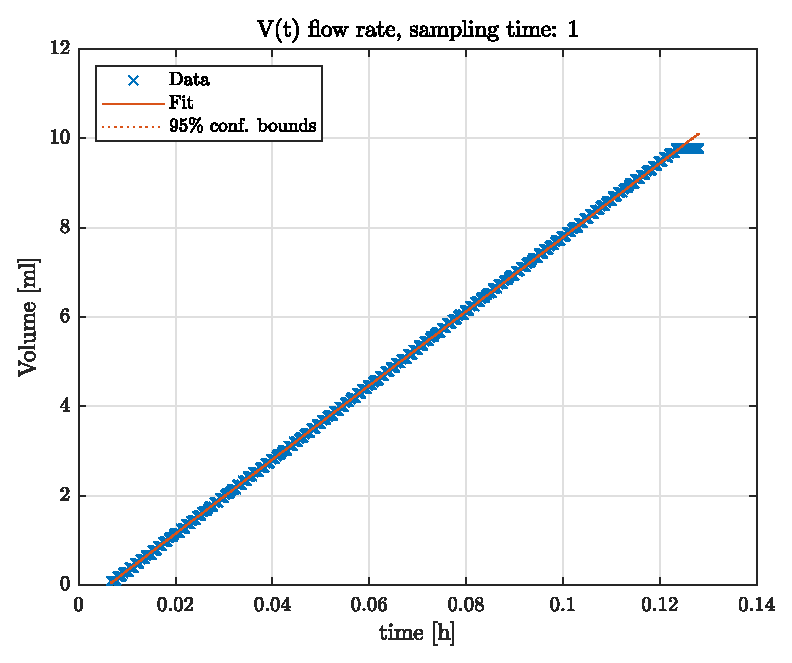
\includegraphics[width=0.8\linewidth]{figures/V_t__flow_rate__sampling_time__1.eps}
		\caption{$V(t)$ of flow rate measurement with sampling time 1s}
		\label{fig:v_t_fr1}
	\end{figure}
	
	\begin{figure}[h!]
		\centering
		\includegraphics[width=0.8\linewidth]{figures/V_t__flow_rate__sampling_time__3.eps}
		\caption{$V(t)$ of flow rate measurement with sampling time 3s}
		\label{fig:v_t_fr3}
	\end{figure}
	
	\newpage
	\begin{figure}[h!]
		\centering
		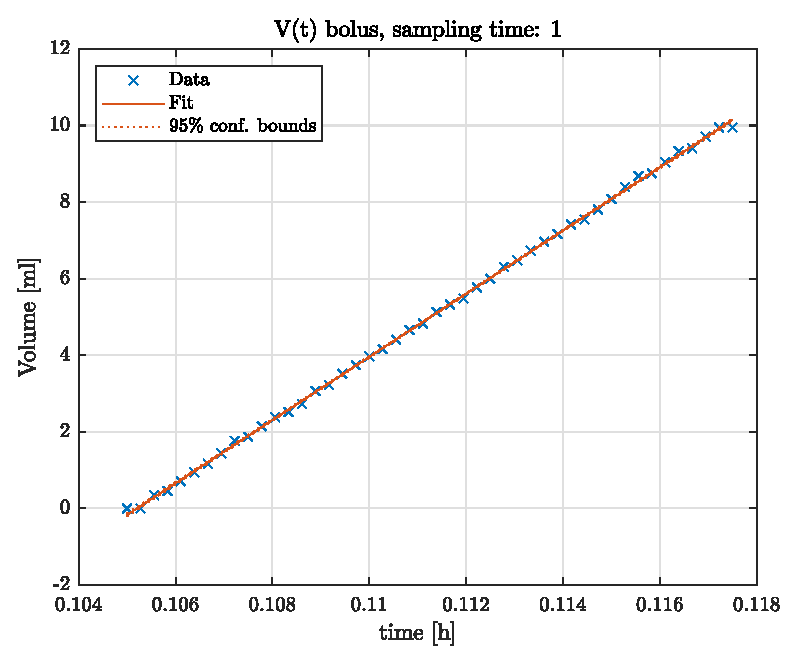
\includegraphics[width=0.8\linewidth]{figures/V_t__bolus__sampling_time__1.eps}
		\caption{$V(t)$ of bolus flow rate measurement with sampling time 1s}
		\label{fig:v_t_bfr1}
	\end{figure}
	
	\begin{figure}[h!]
		\centering
		\includegraphics[width=0.8\linewidth]{figures/V_t__bolus__sampling_time__3.eps}
		\caption{$V(t)$ of bolus flow rate measurement with sampling time 3s}
		\label{fig:v_t_bfr3}
	\end{figure}
	
	\newpage
	\begin{figure}[h!]
		\centering
		\includegraphics[width=0.8\linewidth]{figures/_q__V_inst__t___flow_rate__sampling_time__1.eps}
		\caption{$q_{V,inst}(t)$ of flow rate measurement with sampling time 1s}
		\label{fig:q_t_fr1}
	\end{figure}
	
	\begin{figure}[h!]
		\centering
		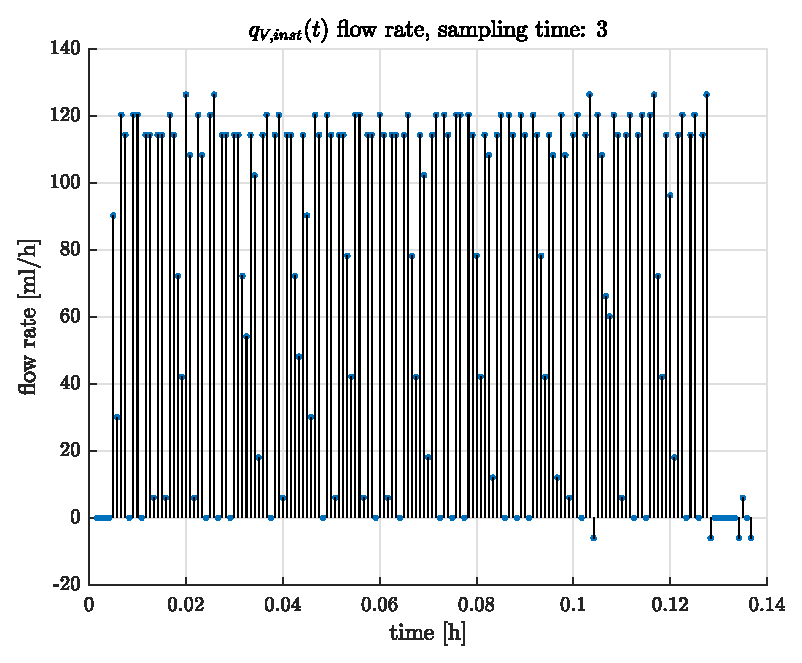
\includegraphics[width=0.8\linewidth]{figures/_q__V_inst__t___flow_rate__sampling_time__3.eps}
		\caption{$q_{V,inst}(t)$ of flow rate measurement with sampling time 3s}
		\label{fig:q_t_fr3}
	\end{figure}
	
	\newpage
	\begin{figure}[h!]
		\centering
		\includegraphics[width=0.8\linewidth]{figures/_q__V_inst__t___bolus__sampling_time__1.eps}
		\caption{$q_{V,inst}(t)$ of bolus flow rate measurement with sampling time 1s}
		\label{fig:q_t_bfr1}
	\end{figure}
	
	\begin{figure}[h!]
		\centering
		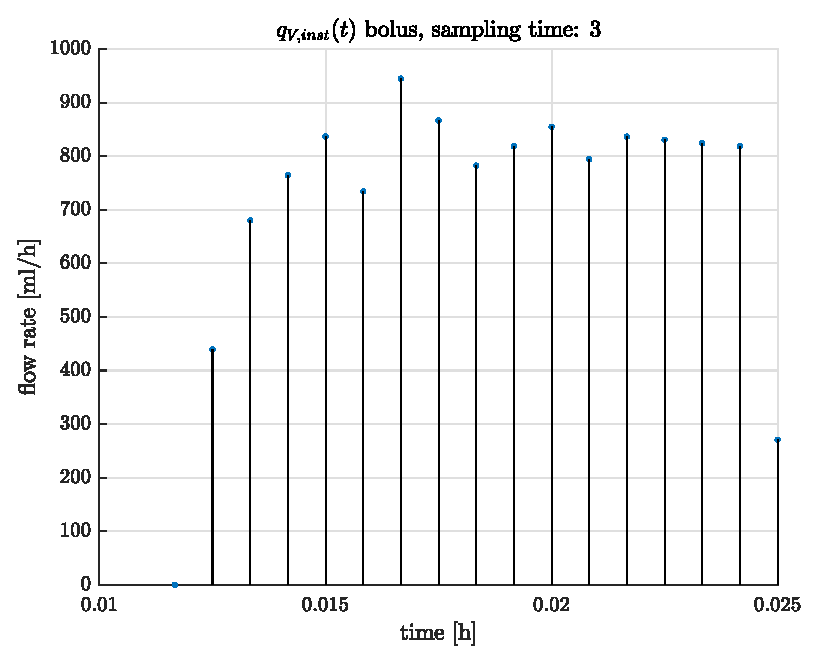
\includegraphics[width=0.8\linewidth]{figures/_q__V_inst__t___bolus__sampling_time__3.eps}
		\caption{$q_{V,inst}(t)$ of bolus flow rate measurement with sampling time 3s}
		\label{fig:q_t_bfr3}
	\end{figure}
	
	\newpage
	To illustrate how volume changed in time plots were drawn. Figures \ref{fig:v_t_fr1} and \ref{fig:v_t_fr3} show the change of the volume in time of flow rate measurement with respectively 1s of sampling time and 3s of sampling time. Next figures describe the same variable yet for bolus measurement with sampling time 1s (Fig. \ref{fig:v_t_bfr1}) and 3s (Fig. \ref{fig:v_t_bfr3}).
	
	In order to emphasize instantaneous flow rate plots of its change in time were created using MATLAB. These can be seen as Figures \ref{fig:q_t_fr1}, \ref{fig:q_t_fr3} for flow rate measurement with sampling time 1s and 3s; and next two Figures \ref{fig:q_t_bfr1}, \ref{fig:q_t_bfr3} are of bolus measurement.
	
	%%%%%%%%%%% FORMULAS AND CALCULATIONS %%%%%%%%%%%%%%%%%
	\section{Formulas and sample calculations}
	
	Calculations of volume based on mass value were done with density equation:
	\begin{equation}\label{d_eq}
		\rho = \frac{m}{V}
	\end{equation}
	\small
	where: \\
	\indent\indent $\rho$ — density of body,\\
	\indent\indent $m$ — mass of body,\\
	\indent\indent $V$ — volume of body
	\normalsize
	\newline
	
	After simple algebra applied:
	\begin{equation}\label{V_eq}
		V = \frac{m}{\rho}
	\end{equation}
	
	Above equation for first mass entry and density of water in 25$\degree C$ (the water temperature was 23.5 $\degree C$, however in table provided by the teacher, 25$\degree C$ was the closest value):
	\begin{equation}\label{V_eg_eq}
		V_{calc} = \frac{9.7450~g}{997.05~\frac{g}{dm^3}} = 0.009773832807~dm^3 \approx 9.77~ml
	\end{equation}
	
	Uncertainty of upper solution:
	\begin{equation}\label{uc_V_eq}
		u_c(V) = \sqrt{\left[\frac{\partial V}{\partial m} u(m)\right]^2 + \left[\frac{\partial V}{\partial \rho} u(\rho)\right]^2} = \sqrt{\left[\frac{1}{\rho} u(m)\right]^2 + \left[-\frac{m}{\rho^2} u(\rho)\right]^2}
	\end{equation}
	\small
	where: \\
	\indent\indent $u(m) = \frac{0.005~g}{\sqrt{3}}$\\
	\indent\indent $u(\rho) = \frac{0.01~\frac{g}{dm^3}}{\sqrt{3}}$
	\normalsize
	\newline
	
	Exemplary calculation of previously defined uncertainty:
	\begin{equation}\label{uc_V_eq_eg}
	\begin{split}
		u_c(V) & = \sqrt{\left[\frac{1}{997.05~\frac{g}{dm^3}} \cdot 0.0029~g\right]^2 + \left[-\frac{9.7450~g}{(997.05~\frac{g}{dm^3})^2}\cdot 0.01~\frac{g}{dm^3}\right]^2}=\\
		& = 0.000002896 dm^3 \approx 0.01 ml
	\end{split}
	\end{equation}
	
	Difference between final and initial syringe volume read from its body:
	\begin{equation}\label{diff_Vs_eq}
		\Delta V_S = V_{S_f} - V_{S_i}
	\end{equation}
	\small
	where: \\
	\indent\indent $V_{S_f}$ — final volume of the syringe,\\
	\indent\indent $V_{S_i}$ — initial volume of the syringe
	\normalsize
	\newline
	
	Example of application of upper formula:
	\begin{equation}\label{diff_Vs_eg_eq}
		\Delta V_S = 39~ml - 29~ml = 10~ml	
	\end{equation}
	
	Uncertainty of syringe volume:
	\begin{equation}\label{uc_diff_Vs_eq}
		u(\Delta V_S) = \frac{1~ml}{\sqrt[]{3}}
	\end{equation}
	
	When it comes to average mass flow rate, following equation was used:
	\begin{equation}\label{qm,avg_eq}
		q_{m,avg} = \frac{m}{t}
	\end{equation}
	\small{
	where: \\
	\indent\indent $m$ — mass of fluid delivered by the pump,\\
	\indent\indent $t$ — time during which the mass was delivered
	}
	\normalsize
	\newline
	
	Exemplary calculations of average mass flow rate:
	\begin{equation}\label{qm,avg_eg_eq}
		q_{m,avg} = \frac{9.7450~g}{440~s} = 0.022147727~\frac{g}{s} \approx 79.73 ~\frac{g}{h}
	\end{equation}
	
	Uncertainty of average mass flow rate is given by following formula:
	\begin{equation}\label{uc_qm,avg_eq}
		u_c(q_{m,avg}) = \sqrt{\left[\frac{\partial q_{m,avg}}{\partial m} u(m)\right]^2 + \left[\frac{\partial q_{m,avg}}{\partial t} u(t)\right]^2} = \sqrt{\left[\frac{1}{t} u(m)\right]^2 + \left[-\frac{m}{t^2} u(t)\right]^2}
	\end{equation}
	\small{
	where: \\
	\indent\indent $u(m)$ — defined as above in \ref{uc_V_eq},\\
	\indent\indent $u(t)$ — assumed a very small number, because it is hard to define it
	}
	\normalsize
	\newline
	
	Followed by an exemplary calculation:
	\begin{equation}\label{uc_qm,avg_eq_eg}
	\begin{split}
		u_c(q_{m,avg}) & = \sqrt{\left[\frac{1}{440~s} \cdot 0.0029~g\right]^2 + \left[-\frac{9.7450~g}{(440~s)^2} \cdot 0.001~s\right]^2} =\\
		& = 0.000006561 \frac{g}{s} \approx 0.66 \frac{g}{h}
	\end{split}
	\end{equation}
	
	Instantaneous mass flow rate was obtained in following way:
	\begin{equation}\label{qm,inst_eq}
		q_{m,inst} = \frac{dm}{dt}
	\end{equation} 
	
	In case of both average and instantaneous volumetric flow rate, formulae \ref{qm,avg_eq}, \ref{uc_qm,avg_eq}, \ref{qm,inst_eq} were used, however instead of $m$ volume $V$ was nominator variable.
	
	\begin{equation}\label{qv,avg_eq}
		q_{V,avg} = \frac{V}{t}
	\end{equation}
	
	\begin{equation}\label{qv,inst_eq}
		q_{V,inst} = \frac{dV}{dt}
	\end{equation}
	
	Average flow rate of instantaneous results is given by:
	\begin{equation}\label{qv,avg,inst_eq}
		q_{V,avg,inst} = \frac{\sum_{k=1}^{n}\frac{dV_k}{dt_k}}{n}
	\end{equation}
	
	
	%%%%%%%%%%% ANALYSIS AND CONCLUSIONS %%%%%%%%%%%%%%%%%%%
	\section{Analysis and Conclusions}
	
	The goal of this work is to determine whether the accuracy of the Braun Perfusor\textsuperscript{\tiny\textregistered} compact syringe pump of both volume and flow rate is as specified by the producer. Flow accuracy given by the producer of this pump is $\pm 2\%$ (measurement time $>$ 1h, min 2 ml). In Tables \ref{tab:uc_flow_rate}, \ref{tab:uc_bolus_flow_rate} values of this uncertainty for samples of this experiment (Tables \ref{tab:flow_rate}, \ref{tab:bolus_flow_rate}) are given. One can see that values of flow rate measurement (Tables \ref{tab:flow_rate}, \ref{tab:uc_flow_rate}) are in fact in range of the accuracy of the set flow rate: \\
	\indent\indent flow rate: $\dot{q_V} = 80.00 \pm 0.92~ml$, mean of calculated volume: $m_{q_{v,calc}} = 80.33 \pm 0.65~ml$.
	
	However, bolus function values of flow rate are out of the range of device accuracy:\\
	\indent\indent bolus flow rate: $\dot{q_{V,b}} = 800.00 \pm 9.24~ml$, mean of calculated volume: $m_{q_{v,b,calc}} = 754.85 \pm 56.614~ml$
	
	Due to the fact that the accuracy of the calculated flow rate for bolus function of the pump is very high --- $7.5\%$ of value, stating that the device in inaccurate would be unreasonable. So, let's just say that the experiment procedure does not allow, due to the high inaccuracy of the measurement, to conclude anything about the device's flow rate of bolus function. On the other hand, normal flow rate option for dosage volume = $10~ml$ and flow rate set to $80~ml$ can be stated to be accurate. The upper bound of the accuracy of the device's flow rate is slightly crossed ($80.92~ml < 80.98~ml$) but this is very small value ($<0.001$) relative to the device's flow rate upper boundary.\\
	
	Volumetric accuracy of the device is $\pm 1$ ml (look at Table \ref{tab:flow_rate_volume}). All of the results of calculated volume fall in range of the inaccuracy of the device. Mean of those is:\\
	\indent\indent $m_{V_{calc}} = 9.98 \pm 0.01~ml$, volume set: $\dot{V}= 10.00 \pm 1.00~ml$.
	
	The accuracy of the device when it comes to the volume delivered is very high: standard deviation of 4 measurements is $\approx 0.15~ml$ what is $15\%$ of provided uncertainty of  $1~ml$. \\
	
	The influence of the sampling time can be seen on volume change in time plots on Figures \ref{fig:v_t_fr1}, \ref{fig:v_t_fr3}, \ref{fig:v_t_bfr1}, \ref{fig:v_t_bfr3}. Having 1s time of sampling there are more points of data what is beneficial for the linear regression model, 95\% conf. bounds are much lower for large amount of points (observed clearly at Fig. \ref{fig:v_t_bfr3}).
	
	Flow rate change in time plots with different sampling time (1s or 3s), presented on Figures \ref{fig:q_t_fr1}, \ref{fig:q_t_fr3}, \ref{fig:q_t_bfr1}, \ref{fig:q_t_bfr3}. Looking at Figure \ref{fig:q_t_fr1}, a lot of point with $q=0$ or $q<0$ can be seen, what is the main difference between 1s sampling time and 3s sampling time presented on Figure \ref{fig:q_t_fr3}, where much less points of this kind are present. Moreover plots for sampling time 3s tend to be more stable, alternations of the flow rate values are smaller than for sampling time 1s plots.
	
	\section{Appendix}
	Following link of github repository serves the MATLAB code and excel data, both were the basis of this work.
	\href[]{}{}
	
\end{document}
